% Copyright 2004 by Till Tantau <tantau@users.sourceforge.net>.
%
% In principle, this file can be redistributed and/or modified under
% the terms of the GNU Public License, version 2.
%
% However, this file is supposed to be a template to be modified
% for your own needs. For this reason, if you use this file as a
% template and not specifically distribute it as part of a another
% package/program, I grant the extra permission to freely copy and
% modify this file as you see fit and even to delete this copyright
% notice. 

\documentclass[aspectratio=169]{beamer}
%\documentclass{beamer}

\setbeamersize{text margin left=10mm, text margin right=10mm}

\defbeamertemplate{headline}{my header}{%
\vskip1pt%
\makebox[0pt][l]{\,\insertshortauthor}%
\hspace*{\fill}\insertshorttitle/\insertshortsubtitle\hspace*{\fill}%
\llap{\insertpagenumber/\insertpresentationendpage\,}
}
\setbeamertemplate{headline}[my header]

\usepackage{soul}
\usepackage{tkz-euclide}
\usetikzlibrary{calc}
\usepackage[]{algorithm2e}
\usepackage{changepage}
\usepackage{amssymb}
\usepackage{xcolor}
\usepackage{mathtools}
\usepackage{tcolorbox}
\usepackage{tikz}
\usetikzlibrary{arrows}
\usepackage{tikz-3dplot}
\usepackage{tkz-euclide}
\usepackage{circuitikz}
\usepackage{pgfplots}
\pgfplotsset{width=7cm,compat=1.8}

\usetikzlibrary{positioning}
% \usepackage[math]{cellspace}
% \cellspacetoplimit 4pt
% \cellspacebottomlimit 4pt
%\usetikzlibrary{arrows.meta}


%\setbeamertemplate{itemize items}{-}

%\usepackage{helvet}
\usefonttheme{professionalfonts} % using non standard fonts for beamer
%\usefonttheme{serif} % default family is serif
%\usepackage{fontspec}
%\setmainfont{Liberation Serif}

% There are many different themes available for Beamer. A comprehensive
% list with examples is given here:
% http://deic.uab.es/~iblanes/beamer_gallery/index_by_theme.html
% You can uncomment the themes below if you would like to use a different
% one:
%\usetheme{AnnArbor}
%\usetheme{Antibes}
%\usetheme{Bergen}
%\usetheme{Berkeley}
%\usetheme{Berlin}
%\usetheme{Boadilla}
%\usetheme{boxes}
%\usetheme{CambridgeUS}
%\usetheme{Copenhagen}
%\usetheme{Darmstadt}
%\usetheme{default}
%\usetheme{Frankfurt}
%\usetheme{Goettingen}
%\usetheme{Hannover}
%\usetheme{Ilmenau}
%\usetheme{JuanLesPins}
%\usetheme{Luebeck}
%\usetheme{Madrid}
%\usetheme{Malmoe}
%\usetheme{Marburg}
%\usetheme{Montpellier}
%\usetheme{PaloAlto}
%\usetheme{Pittsburgh}
%\usetheme{Rochester}
%\usetheme{Singapore}
%\usetheme{Szeged}
%\usetheme{Warsaw}

\def\mf{\ensuremath\mathbf}
\def\mb{\ensuremath\mathbb}
\def\lp{\ensuremath\left(}
\def\rp{\ensuremath\right)}
\def\lv{\ensuremath\left\lvert}
\def\rv{\ensuremath\right\rvert}
\def\lV{\ensuremath\left\lVert}
\def\rV{\ensuremath\right\rVert}
\def\lc{\ensuremath\left\{}
\def\rc{\ensuremath\right\}}
\def\bmx{\ensuremath\begin{bmatrix*}[r]}
\def\emx{\ensuremath\end{bmatrix*}}

\newcommand{\demoex}[2]{\onslide<#1->\begin{color}{black!60} #2 \end{color}}

\title{Linear Systems}

% A subtitle is optional and this may be deleted
\subtitle{Eigenvalues and Eigenvectors}

\author{Sivakumar Balasubramanian}
% - Give the names in the same order as the appear in the paper.
% - Use the \inst{?} command only if the authors have different
%   affiliation.

\institute[Christian Medical College] % (optional, but mostly needed)
{
  \inst{}%
  Department of Bioengineering\\
  Christian Medical College, Bagayam\\
  Vellore 632002
}
% - Use the \inst command only if there are several affiliations.
% - Keep it simple, no one is interested in your street address.

\date{}
% - Either use conference name or its abbreviation.
% - Not really informative to the audience, more for people (including
%   yourself) who are reading the slides online

\subject{Lecture notes on linear systems}
% This is only inserted into the PDF information catalog. Can be left
% out. 

% If you have a file called "university-logo-filename.xxx", where xxx
% is a graphic format that can be processed by latex or pdflatex,
% resp., then you can add a logo as follows:

% \pgfdeclareimage[height=0.5cm]{university-logo}{university-logo-filename}
% \logo{\pgfuseimage{university-logo}}

% Delete this, if you do not want the table of contents to pop up at
% the beginning of each subsection:
\AtBeginSubsection[]
{
  \begin{frame}<beamer>{Outline}
    \tableofcontents[currentsection,currentsubsection]
  \end{frame}
}

% Let's get started
\begin{document}

\pgfplotsset{
  compat=1.8,
  colormap={whitered}{color(0cm)=(white); color(1cm)=(orange!75!red)}
}


\begin{frame}
  \titlepage
\end{frame}

\begin{frame}[t]{References}
\begin{itemize}
    \item G Strang, Linear Algebra: Chapters 5.
\end{itemize} 
\end{frame}


\begin{frame}[t]{Linear transformation}
\begin{itemize}
    \item Matrices represent linear transformations, $\mf{A} \in \mb{R}^{m \times n}$ represents a transformation $T: \mb{R}^n \to \mb{R}^m$. 
    \[ \mf{y} = T\left(\mf{x}\right) = \mf{A}\mf{x}, \,\,\,\, \mf{x} \in \mb{R}^n \text{ and } \, \mf{y} \in \mb{R}^m \]

    \item Consider a linear transformation $T: \mb{R}^n \to \mb{R}^n$.

    In general, $T$ scales and rotates the vector $\mf{x}$ to produce $\mf{y}$.

    \begin{center}
    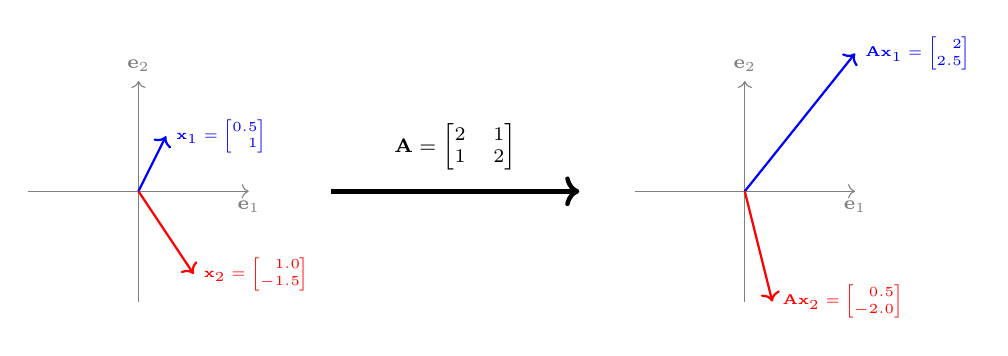
\begin{tikzpicture}[scale=0.7]
    \draw[thin, gray, ->] (-2,0) -- (2, 0) node[below] {\scriptsize{$\mf{e}_1$}};
    \draw[thin, gray, ->] (0, -2) -- (0, 2) node[above] {\scriptsize{$\mf{e}_2$}};
    \draw[thick, blue, ->] (0, 0) -- (0.5, 1) node[right] {\tiny{$\mf{x}_1 = \begin{bmatrix*}[r]0.5\\1\end{bmatrix*}$}};
    \draw[thick, red, ->] (0, 0) -- (1, -1.5) node[right] {\tiny{$\mf{x}_2 = \begin{bmatrix*}[r]1.0\\-1.5\end{bmatrix*}$}};

    \draw[ultra thick, black, ->] (3.5, 0) -- (8.0, 0);

    \node[black, above] at (5.75, 0.2) {\scriptsize{$\mf{A} = \begin{bmatrix*}2 & 1\\1 & 2\end{bmatrix*}$}};

    \draw[thin, gray, ->] (9,0) -- (13, 0) node[below] {\scriptsize{$\mf{e}_1$}};
    \draw[thin, gray, ->] (11, -2) -- (11, 2) node[above] {\scriptsize{$\mf{e}_2$}};
    \draw[thick, blue, ->] (11, 0) -- (13, 2.5) node[right] {\tiny{$\mf{A}\mf{x}_1 = \begin{bmatrix*}[r]2\\2.5\end{bmatrix*}$}};
    \draw[thick, red, ->] (11, 0) -- (11.5, -2.0) node[right] {\tiny{$\mf{A}\mf{x}_2 = \begin{bmatrix*}[r]0.5\\-2.0\end{bmatrix*}$}};
    \end{tikzpicture}
    \end{center}

\end{itemize}
\end{frame}


\begin{frame}[t]{Linear transformation}

{\small{An easier way is to look at what happens to the standard basis $\left\{\mf{e}_i\right\}_{i=1}^{n}$.}}

\begin{center}
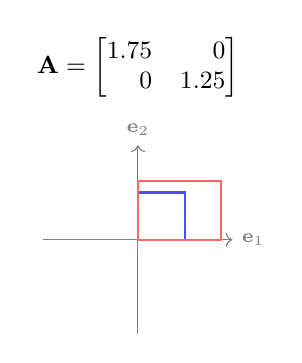
\begin{tikzpicture}[scale=0.6]
\draw[thin, gray, ->] (-2,0) -- (2, 0) node[right] {\scriptsize{$\mf{e}_1$}};
\draw[thin, gray, ->] (0, -2) -- (0, 2) node[above] {\scriptsize{$\mf{e}_2$}};

\draw[thick, blue!70!, -] (0, 0) -- (1, 0) -- (1, 1) -- (0, 1) -- (0,0);
\draw[thick, red!60!, -] (0, 0) -- (1.75, 0) -- (1.75, 1.25) -- (0, 1.25) -- (0, 0);

\node[below, black] at (0.0, 4.5) {\small{$\mf{A} = \begin{bmatrix*}[r]1.75 & 0\\0 & 1.25\end{bmatrix*}$}};
\end{tikzpicture} \hspace{0.1cm}
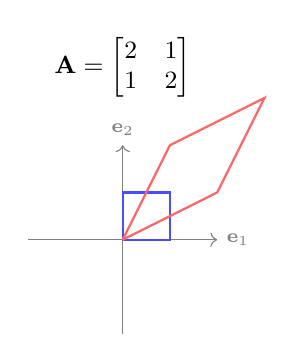
\begin{tikzpicture}[scale=0.6]
\draw[thin, gray, ->] (-2,0) -- (2, 0) node[right] {\scriptsize{$\mf{e}_1$}};
\draw[thin, gray, ->] (0, -2) -- (0, 2) node[above] {\scriptsize{$\mf{e}_2$}};
\draw[thick, blue!70!, -] (0, 0) -- (1, 0) -- (1, 1) -- (0, 1) -- (0,0);

\draw[thick, red!60!, -] (0, 0) -- (2, 1) -- (3, 3) -- (1, 2) -- (0, 0);

\node[below, black] at (0.0, 4.5) {\small{$\mf{A} = \begin{bmatrix*}2 & 1\\1 & 2\end{bmatrix*}$}};
\end{tikzpicture} \hspace{0.1cm}
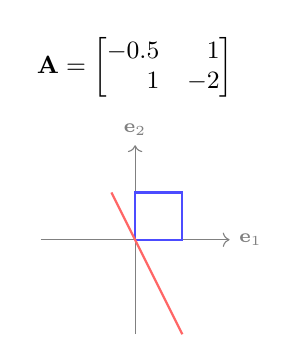
\begin{tikzpicture}[scale=0.6]
\draw[thin, gray, ->] (-2,0) -- (2, 0) node[right] {\scriptsize{$\mf{e}_1$}};
\draw[thin, gray, ->] (0, -2) -- (0, 2) node[above] {\scriptsize{$\mf{e}_2$}};
\draw[thick, blue!70!, -] (0, 0) -- (1, 0) -- (1, 1) -- (0, 1) -- (0,0);

\draw[thick, red!60!, -] (0, 0) -- (-0.5, 1) -- (0.5, -1) -- (1, -2) -- (0, 0);

\node[below, black] at (0.0, 4.5) {\small{$\mf{A} = \begin{bmatrix*}[r]-0.5 & 1\\1 & -2\end{bmatrix*}$}};
\end{tikzpicture} \hspace{0.1cm}
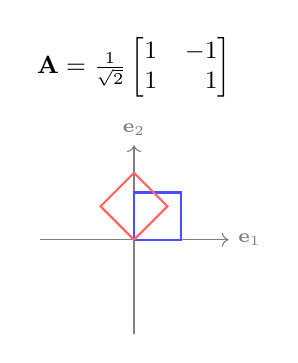
\begin{tikzpicture}[scale=0.6]
\draw[thin, gray, ->] (-2,0) -- (2, 0) node[right] {\scriptsize{$\mf{e}_1$}};
\draw[thin, gray, ->] (0, -2) -- (0, 2) node[above] {\scriptsize{$\mf{e}_2$}};
\draw[thick, blue!70!, -] (0, 0) -- (1, 0) -- (1, 1) -- (0, 1) -- (0,0);

\draw[thick, red!60!, -] (0, 0) -- (0.707, 0.707) -- (0, 1.414) -- (-0.707, 0.707) -- (0, 0);

\node[below, black] at (0.0, 4.5) {\small{$\mf{A} = \frac{1}{\sqrt{2}}\begin{bmatrix*}[r]1 & -1\\1 & 1\end{bmatrix*}$}};
\end{tikzpicture}
\end{center}

\end{frame}


\begin{frame}[t]{Linear transformation in different basis}
\begin{itemize}
    \item Consider a basis $V=\left\{\mf{v}_i\right\}_{i=1}^{n}$ for $\mb{R}^n$. Let $\mf{x} = \begin{bmatrix*}x_1 & x_2 & \ldots & x_n\end{bmatrix*}^T \in \mb{R}^n$ be the representation of $\mf{x}$ in 
    the standard basis.
    
    Representation of $\mf{x}$ in $V$ is,
    \[ \mf{x}_{V} = \sum_{i=1}^n x_{vi}\mf{v}_i, \,\,\, \mf{x}_V = \begin{bmatrix*}x_{v1} & x_{v2} & \ldots & x_{vn}\end{bmatrix*}^T \]

    \item We can go back and forth between these two representations in the following way,
    \[ \mf{x} = \mf{V}\mf{x}_V \,\,\, \text{ and } \,\,\, \mf{x}_V = \mf{V}^{-1}\mf{x}; \,\,\, \text{where, } \mf{V} = \begin{bmatrix*}\mf{v}_1 & \mf{v}_2 & \ldots & \mf{v}_n\end{bmatrix*} \]

    \item When $V$ is an orthonormal basis, then the algebra gets simpler,
    \[ \mf{x} = \mf{V}\mf{x}_V \,\,\, \text{ and } \,\,\, \mf{x}_V = \mf{V}^T\mf{x} \]

\end{itemize}
\end{frame}


\begin{frame}[t]{Linear transformation in different basis}
\begin{small}
Consider a linear transformation $T: \mb{R}^2 \to \mb{R}^2$ represented by the matrix $\mf{A} = \begin{bmatrix*}[r]2 & 1\\-1 & 1\end{bmatrix*}$. Consider a vector $\mf{x} = \begin{bmatrix*}[r]3\\-1\end{bmatrix*}$. What is $\mf{y} = \mf{Ax}$?

\[ \mf{y} = \mf{Ax} = \begin{bmatrix*}[r]2 & 1\\-1 & 1\end{bmatrix*}\begin{bmatrix*}[r]3\\-1\end{bmatrix*} = \begin{bmatrix*}[r]5\\-4\end{bmatrix*} \]

Now, consider a basis $V = \left\{\begin{bmatrix*}[r]1\\-1\end{bmatrix*}, \begin{bmatrix*}[r]2\\4\end{bmatrix*}\right\}$ for $\mb{R}^2$. The representation of $\mf{x}, \mf{y}$ in $V$ is, 

\[ \mf{x}_V = \mf{V}^{-1}\mf{x} = \frac{1}{6}\begin{bmatrix*}[r]4 & -2\\1 & 1\end{bmatrix*}\begin{bmatrix*}[r]3\\-1\end{bmatrix*} = \frac{1}{6}\begin{bmatrix*}[r]14\\2\end{bmatrix*}, \,\,\, \mf{y}_V = \frac{1}{6}\begin{bmatrix*}[r]28\\1\end{bmatrix*}\]

Now, if we apply the linear transformation $T$ on $\mf{x}_V$ will we get $\mf{y}_V$?

\[ \mf{A}\mf{x}_V = \begin{bmatrix*}[r]2 & 1\\-1 & 1\end{bmatrix*}\frac{1}{6}\begin{bmatrix*}[r]14\\2\end{bmatrix*} = \frac{1}{6}\begin{bmatrix*}[r]16\\-12\end{bmatrix*} \neq \mf{y}_V \]

\textbf{Representation of a linear transformation $T$ is basis dependent! }
\end{small}

\end{frame}


\begin{frame}[t]{Similarity transformation}
\begin{itemize}
    \item Linear transformations represented in one basis represent a different transformation in another basis. This issue can be addressed by keeping track of the basis one is working in.

    \item Let $\mf{x}, \mf{y}$ be representations in the standard basis. Changing basis to $V$, gives us $\mf{x}_V, \mf{y}_V$.
    \[ \mf{y}_V = \mf{V}^{-1}\mf{y} = \mf{V}^{-1}\mf{Ax} = \mf{V}^{-1}\mf{A}\mf{V}\mf{x}_V = \mf{A}_V\mf{x}_V \]
\end{itemize}

\begin{small}
\demoex{2}{
    $\bullet$ Check if this works with the example in the previous slide. $\mf{A} = \begin{bmatrix*}[r]2 & 1\\-1 & 1\end{bmatrix*}$; $\mf{V} = \begin{bmatrix*}[r]1 & 2\\-1 & 4\end{bmatrix*}$. Determine $\mf{A}_V$ and check that $\mf{y}_V = \mf{A}_V\mf{x}_V$.
}\vspace{0.3cm}

\demoex{3}{
    $\bullet$ A linear transformation $\hat{T}$ is represented as $\mf{A}_V$ in $V$. What is its representation in the standard basis? E.g.: $\mf{A}_V = \begin{bmatrix*}[r]-4 & 2\\3 & -5\end{bmatrix*}$; $\mf{V} = \frac{1}{\sqrt{2}}\begin{bmatrix*}[r]1 & 1\\-1 & 1\end{bmatrix*}$. Determine $\mf{A}$. If $\mf{x}_V = \bmx \frac{1}{2} & 2\emx^T$. What is $\mf{y}_V$ and $\mf{y}$?
}
\end{small}
\end{frame}


\begin{frame}[t]{Similarity transformation}
\begin{itemize}
    \item Two matrices $\mf{A}, \mf{B} \in \mb{R}^{n \times n}$ are called \textit{similar} matrices, if there exists a non-singular matrix $\mf{Q}$, such that,
    \[ \mf{B} = \mf{Q}^{-1}\mf{A}\mf{Q} \]

    \item The transformation represented by $\mf{Q}^{-1}\mf{A}\mf{Q}$ is called the \textit{similarity transformation}.

    \item \textit{Similar} matrices represent the same linear transformation in different basis.

    \item When $\mf{Q}$ is an orthogonal matrix, we have $\mf{B} = \mf{Q}^T\mf{A}\mf{Q}$. 
\end{itemize}
\end{frame}


\begin{frame}[t]{Complex Vectors and Matrices}
\begin{itemize}
    \item Similar to $\mb{R}^n$, we can have $\mb{C}^n$. $\mf{x} = \begin{bmatrix*}x_{1}\\x_{2}\\\vdots\\x_{n}\end{bmatrix*} = \begin{bmatrix*}x_{r1} + jx_{i1}\\x_{r2} + jx_{i2}\\\vdots\\x_{rn} + jx_{in}\end{bmatrix*}$
    
    \item Vector addition and scalar mulitplication are the same. The scalar is a complex number.
    
    \item Additive identity, and scalar multiplication identity are the same. So is the \textbf{standard basis} $\left\{\mf{e}_i\right\}_{i=1}^{n}$
    
    \item \textbf{Linear independence}: The set $\left\{\mf{v}_i\right\}_{i=1}^n$ with $\mf{v}_i \in \mb{C}^n$ is linearly independent, if  $\sum_{i=1}^nc_i\mf{v}_i = 0, \implies c_i = 0, \,\, \forall 1 \leq i \leq n, \,\,\, c_i \in \mb{C}$
    
    \item \textbf{Inner product}: $\mf{x}^H\mf{y} = \begin{bmatrix*}\overline{x}_1&\overline{x}_2&\ldots&\overline{x}_n\end{bmatrix*}\begin{bmatrix*}y_1\\y_2\\\vdots\\y_n\end{bmatrix*} = \sum_{i=1}^n\overline{x}_iy_i$

\end{itemize}
\end{frame}


\begin{frame}[t]{Complex Vectors and Matrices}
\begin{itemize}
    \item \textbf{Length}: $\left\lVert \mf{x}\right\rVert_2^2 = \mf{x}^H\mf{x} = \sum_{i=1}^n\overline{x}_ix_i = \sum_{i=1}^n\left\lvert x_i\right\rvert^2$

    \item \textbf{Orthogonality}: $\mf{x}^H\mf{y} = 0$

    \item Complex matrices have complex entries. $\mf{A} \in \mb{C}^{m \times n}$ such that $a_{ij} \in \mb{C}, \,\, \forall 1 \leq i \leq m, \,\, 1 \leq j \leq n$

    \item The transpose operation is generalized to conjugate transpose known as the \textit{Hermitian}. $\mf{A}^H = \overline{\mf{A}}^T$.
    
    \item The idea of symmetric matrices $\mb{R}^{n \times n}$ are now generalized to $\mb{C}^{n \times n}$  as $\mf{A} = \mf{A}^H$. Such matrices are called \textbf{Hermitian} matrices.

    \item Orthogonal matrices in the complex case are called \textbf{Unitary} matrices, $\mf{U}^H\mf{U} = \mf{I} \implies \mf{U}^{-1} = \mf{U}^H$.
\end{itemize}
\end{frame}


\begin{frame}[t]{Eigenvectors and Eigenvalues}
\begin{itemize}
    \item Any linear transformation represented by $\mf{A} \in \mb{C}^{n \times n}$ has vectors that satisfy the following property,
    \[ \mf{Ax} = \lambda \mf{x}, \,\,\,\,\, \mf{x} \in \mb{C}^n, \, \lambda \in \mb{C}, \,\,\, \mf{x} \neq \mf{0} \]
    where, $\lambda$ and $\mf{x}$ are called the eigenvalue and the associated eigenvector of $\mf{A}$.
    
    \item Any such pair $\left(\lambda, \mf{x}\right)$ is called the eigenpair of $\mf{A}$.
    
    \item These are important for understanding and solving linear differential and difference equations:
    \[ \frac{d\mf{x}\left(t\right)}{dt} = \mf{A}\mf{x}\left(t\right) \,\,\, \text{ and } \,\,\, \mf{x}\left[n+1\right] = \mf{A}\mf{x}\left[n\right] \]
\end{itemize}
\end{frame}


\begin{frame}[t]{Eigenvectors and Eigenvalues}
\begin{small}
Consider the differential equation, $\frac{d\mf{x}\left(t\right)}{dt} = \mf{A}\mf{x}\left(t\right) = \begin{bmatrix*}2 & 1\\1 & 4\end{bmatrix*}\mf{x}\left(t\right)$. Let us assume that the solution is of the form, $\mf{x} = e^{\lambda t}\hat{\mf{x}}$. Then we have,
\[ \frac{d\mf{x}\left(t\right)}{dt} = e^{\lambda t}\mf{A}\hat{\mf{x}} = e^{\lambda t} \lambda \hat{\mf{x}} \implies \mf{A}\hat{\mf{x}} = \lambda \hat{\mf{x}} \]
\[ \begin{bmatrix*}2 & 1\\1 & 4\end{bmatrix*}\begin{bmatrix*}\hat{x}_1\\\hat{x}_2\end{bmatrix*} = \begin{bmatrix*}\lambda \hat{x}_1\\\lambda \hat{x}_2\end{bmatrix*} \implies \begin{bmatrix*}2 - \lambda & 1\\1 & 4 - \lambda\end{bmatrix*}\begin{bmatrix*}\hat{x}_1\\\hat{x}_2\end{bmatrix*} = \begin{bmatrix*}0\\0\end{bmatrix*} \]
where, $\hat{\mf{x}} \in N\left(\mf{A} - \lambda\mf{I}\right)$.
\vspace{0.2cm}

This problem can be solved by, $\det \left(\mf{A} - \lambda\mf{I}\right) = \left\lvert\mf{A} - \lambda\mf{I}\right\rvert = 0$
\[ \left(2 - \lambda\right)\left(4 - \lambda\right) - 1  = \lambda^2 - 6\lambda + 7 = 0 \implies \lambda = 3 \pm \sqrt{2} \]
\[ \mf{A}\hat{\mf{x}} = \left(3 + \sqrt{2}\right) \hat{\mf{x}} \implies \hat{\mf{x}} =  \begin{bmatrix*}-1 + \sqrt{2}\\1\end{bmatrix*} \,\,\, \text{ and } \,\,\, \mf{A}\hat{\mf{x}} = \left(3 - \sqrt{2}\right) \hat{\mf{x}} \implies \hat{\mf{x}} =  \begin{bmatrix*}-1 - \sqrt{2}\\1\end{bmatrix*} \]
$\left(3 + \sqrt{2}, \begin{bmatrix*}-1 + \sqrt{2}\\1\end{bmatrix*}\right)$ and $\left(3 - \sqrt{2}, \begin{bmatrix*}-1 - \sqrt{2}\\1\end{bmatrix*}\right)$ are the eigenpairs of $\mf{A}$.
\end{small}
\end{frame}


\begin{frame}[t]{Eigenvalues and Eigenvectors}

\begin{itemize}
    \item We can find the eigenpairs using the same approach for $\mf{A} \in \mb{C}^{n \times n}$, $\det \left(\mf{A} - \lambda\mf{I}\right) = 0 = p\left(\lambda\right)$.

    \item $p\left(\lambda\right)$ is the characteristic polynomial of $\mf{A}$, and $p\left(\lambda\right) = 0$ is the characteristic equation.

    \item The eigenvalues are the roots of the polynomial $p\left(\lambda \right)$, and the $\mf{x}$ in $\left(\mf{A} - \lambda\mf{I}\right)\mf{x} = 0$ for the different $\lambda$s are the corresponding eigenvectors. 

    \item The subspace spanned by $\mf{x}$ for a particular $\lambda$ is called the eigenspace.

    \item $\mf{A}$ has $n$ eigenvalues, some of which can be complex, and some might be repeated.

    \item For a real matrix, all complex eigenvalues occur in conjugate pairs.
\end{itemize}

\demoex{2}{
    Compute the eigenpairs for the following matrices: $\bmx2 & 1\\-1 & 3\emx$, $\bmx1 & 0\\0 & 1\emx$, $\bmx2 & 1\\ 1 & 2\emx$, $\bmx\frac{\sqrt{3}}{2} & \frac{1}{2}\\-\frac{1}{2} & \frac{\sqrt{3}}{2}\emx$, $\bmx 0 & -2\\2 & 0\emx$
}
\end{frame}


\begin{frame}[t]{Diagonalization of a matrix}

Often the right choice of basis can simplify an equation or the analysis of a problem. For example,
\begin{columns}
\begin{column}{0.5\textwidth}
    \begin{center}
        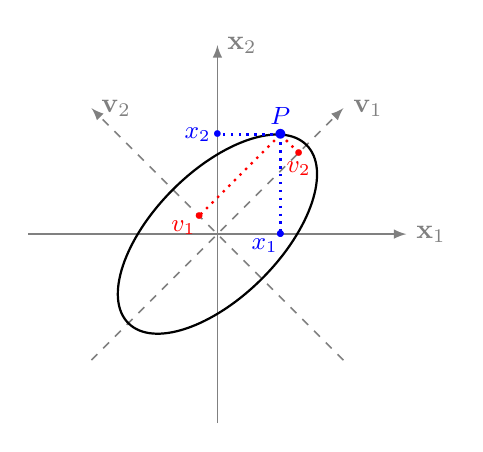
\begin{tikzpicture}[scale=0.8]
        \draw[gray, -latex, line width=0.2mm] (-3, 0) -- (3, 0) node[right] {$\mf{x}_1$};
        \draw[gray, -latex, line width=0.2mm] (0, -3) -- (0, 3) node[right] {$\mf{x}_2$};
        \draw[gray, dashed, -latex, line width=0.2mm] (-2, -2) -- (2, 2) node[right] {$\mf{v}_1$};
        \draw[gray, dashed, -latex, line width=0.2mm] (2, -2) -- (-2, 2) node[right] {$\mf{v}_2$};
        \draw[thick, rotate=45] (0,0) ellipse (2 and 1);
        \node[blue, above] at (1, 1.579795) {\small{${P}$}};
        \draw[blue, dotted, line width=0.3mm] (1, 1.579795) -- (1, 0) node[blue, yshift=-0.15cm, xshift=-0.2cm] {\small{$x_1$}};
        \node[blue] at (1, 0) {\tiny{$\bullet$}};
        \draw[blue, dotted, line width=0.3mm] (1, 1.579795) -- (0, 1.579795) node[blue, xshift=-0.25cm, yshift=0.cm] {\small{$x_2$}}; 
        \node[blue] at (0, 1.579795) {\tiny{$\bullet$}};
        \draw[red, dotted, line width=0.3mm] (1, 1.579795) -- (-0.289892, 0.289892) node[red, yshift=-0.15cm, xshift=-0.2cm] {\small{$v_1$}};
        \node[red] at (-0.289892, 0.289892) {\tiny{$\bullet$}};
        \draw[red, dotted, line width=0.3mm] (1, 1.579795) -- (1.289897, 1.289897) node[red, yshift=-0.2cm, xshift=0.0cm] {\small{$v_2$}};
        \node[blue] at (1, 0) {\tiny{$\bullet$}};
        \node[red] at (1.289897, 1.289897) {\tiny{$\bullet$}};
        \node[blue] at (1, 1.579795) {\small{$\bullet$}};
        % \draw[blue, dotted, line width=0.5mm] (1, 1.579795) -- (0, 1.579795); 
        \end{tikzpicture}
    \end{center}
\end{column}
\begin{column}{0.5\textwidth}
The equation of the ellipse in standard basis is: 
\[ 3x_1^2 + 3x_2^2 - 2x_1x_2 = 1 \]

This has a much simpled representation in the dashed coordinate frame. 
\[ 4v_1^2 + 2v_2^2 = 1 \]

The use of similarity transformation to simplify a matrix is at the heart of diagonalization.
\end{column}
\end{columns}
\end{frame}


\begin{frame}[t]{Diagonalization of a matrix}
\begin{itemize}
    \item Consider a matrix $\mf{A}$ with $n$ eigenpairs $\left\{\left(\lambda_i, \mf{x}_i\right)\right\}_{i=1}^n$.
    \[ \mf{A}\begin{bmatrix*}\mf{x}_1 & \mf{x}_2 & \ldots & \mf{x}_n\end{bmatrix*} = \begin{bmatrix*}\lambda_1\mf{x}_1 & \lambda_2\mf{x}_2 & \ldots & \lambda_n\mf{x}_n\end{bmatrix*} \]
    \[ \mf{AX} = \mf{X}\begin{bmatrix*}\lambda_1 & 0 & \ldots & 0\\0 & \lambda_2 & \ldots & 0\\\vdots & \vdots & \ddots & \vdots\\0 & 0 & \ldots & \lambda_n\end{bmatrix*} = \mf{X}\mf{\Lambda} \]

    \item If the eignevectors are linearly independent, then we have $\mf{X}^{-1}\mf{A}\mf{X} = \mf{\Lambda}$
\end{itemize}

\demoex{2}{
    Let $T: \mb{R}^2 \to \mb{R}^2$ represented by $\mf{A} = \bmx 8 & 1\\2 & 7\emx$. Diagonalize this matrix. What does $\mf{A}$ do to $\mf{x} = \bmx 3 & 4\emx^T$?
}\vspace{0.2cm}

\demoex{3}{
    What about $\mf{A} = \bmx 3 & -1\\-1 & 3\emx$?
}
\end{frame}


\begin{frame}[t]{Diagonalization of a matrix: Eigenpairs of special matrices}
\begin{itemize}
    \item A square matrices with a complete set of eigenvectors, i.e. a linearly independent set of $n$ eigenvectors, can be decomposed into the following,
    \[ \mf{A} = \mf{X}\mf{\Lambda}\mf{X}^{-1} \]

    \item When $\mf{A} \in \mb{R}^{n \times n}$ is symmetric, i.e. $\mf{A} = \mf{A}^T$,
    \begin{itemize}
        \item All eigenvalues are real.
        \item The matrix poses a complete set of eigenvectors, i.e. they form a linearly independent set.
        \item The eigenvectors can be chosen to be orthogonal to each other. When the eigenvalues are distinct, the eigenvectors are orthogonal. But when the eigenvalues are not distinct, we can choose them to be orthogonal.
    \end{itemize}
    This gives us, $\mf{A} = \mf{A}^T = \mf{X}\mf{\Lambda}\mf{X}^T$.
\end{itemize}

\demoex{2}{
    Diagonalize $\mf{A} = \bmx 0 & 1 & 0\\1 & 0 & 0\\0 & 0 & 1\emx$.
}\vspace{0.2cm}
\end{frame}


\begin{frame}[t]{Diagonalization of a matrix}
\begin{itemize}
    \item A change of basis to $\mf{X}$ simplifies $\mf{A}$ to a diagonal matrix, the simplest possible form.

    \item If a matrix $\mf{A}$ has $n$ distinct eigenvalues, then $\mf{A}$ can always be diagonalized.

    \item When there are repeated eigenvalues, we might not always be able to diagonalize a matrix. This happens when there aren't enough eigenvectors. These are called \textit{defective} matrices.
    \[ \text{Algebraic multiplicity} \neq \text{Geometric multiplicity} \]
    where, \textit{algebraic multiplicity} is the number of times the eigenvalue $\lambda$ is repeated, and \textit{geometric multiplicity} is $\dim N\lp \mf{A} - \lambda\mf{I}\rp$.
\end{itemize}

\demoex{2}{
    Diagonalize $\mf{A} = \bmx 1 & 2\\0 & 1\emx$.
}\vspace{0.2cm}

\end{frame}


\begin{frame}[t]{Jordan Form}
\begin{itemize}
    \item If $\mf{A}$ cannot be diagonalized, the next best thing is the \textit{Jordan form}.

    \item Let $\mf{A}$ have eigenvalues $\left(\lambda_1, \lambda_2, \ldots \lambda_k\right)$. We can find a similarity transformation, such that,
    \[ \mf{A} = \mf{P}\mf{J}\mf{P}^{-1}, \,\,\, \mf{J} = \begin{bmatrix*}
    \mf{J}\left(\lambda_1\right) & \mf{0} & \ldots & \mf{0}\\
    \mf{0} & \mf{J}\left(\lambda_2\right) & \ldots & \mf{0}\\
    \vdots & \vdots & \ddots & \vdots\\
    \mf{0} & \mf{0} & \ldots & \mf{J}\left(\lambda_k\right)\\
    \end{bmatrix*} \]
\end{itemize}
\begin{columns}
\begin{column}{0.5\textwidth}
\begin{footnotesize}
Each $\mf{J}\left(\bullet\right)$ is associated with an eigenvalue and an eigenvector, and  is called a Jordan block, and has the form
\[ \mf{J}\left(\lambda_l\right) = \begin{bmatrix*}
\lambda_l & 1 & 0 & \ldots & 0 \\
0 & \lambda_l & 1 & \ldots & 0 \\
0 & 0 & \lambda_l & \ldots & 0 \\
\vdots & \vdots & \vdots & \ddots & 1 \\
0 & 0 & 0 & \ldots & \lambda_l \\
\end{bmatrix*} \]
\end{footnotesize}
\end{column}
\begin{column}{0.5\textwidth}
\begin{footnotesize}
\begin{itemize}
    \item $\mf{J} \in \mb{C}^{r \times r}$. $r$ = the algebraic multiplicity of the eigenvalue $\lambda_l$.
    \item $1$ = the geometric multiplicity of the eigenvalue $\lambda_l$ = $\dim N\left(\mf{A} - \lambda_l\mf{I}\right)$.
    \item A 1-by-1 Jordan block is simply $[\lambda_l]$, corresponding to a eigenvalue with an associated eigenvector.
\end{itemize}
\end{footnotesize}
\end{column}
\end{columns}
\end{frame}


\begin{frame}[t]{Jordan Form}
\begin{small}
\demoex{1}{
    $\bullet$ Jordan form of a diagonalizable matrix $\mf{A} \rightarrow \mf{J} = \bmx
    \lambda_1 & 0 & \ldots & 0\\
    0 & \lambda_2 & \ldots & 0\\
    \vdots & \vdots & \ddots & 0\\
    0 & 0 & \ldots & \lambda_n
    \emx$
}

\demoex{2}{
    $\bullet$ $\lambda = -2$ (AM\footnote{AM: Algebraic multiplicity} = 1, GM\footnote{GM: Geometric multiplicity} = 1), and $\lambda = 11$ (AM = 2, GM = 1) $\rightarrow \mf{J} = \bmx
    -2 & 0 & 0\\
    0 & 11 & 1\\
    0 & 0 & 11
    \emx$
}

\demoex{3}{
    $\bullet$ Write down the Jordan form.\\$\lambda_1 = 1$ (AM = 2, GM = 1)\\$\lambda_2 = 11$ (AM = 3, GM = 2)\\$\lambda_3 = 0$ (AM = 3, GM = 1)\\$\lambda_4 = -1$ (AM = 2, GM = 2). 
}
\end{small}
\end{frame}


\end{document}